% ****** Start of file apssamp.tex ******
%
%   This file is part of the APS files in the REVTeX 4.2 distribution.
%   Version 4.2a of REVTeX, December 2014
%
%   Copyright (c) 2014 The American Physical Society.
%
%   See the REVTeX 4 README file for restrictions and more information.
%
% TeX'ing this file requires that you have AMS-LaTeX 2.0 installed
% as well as the rest of the prerequisites for REVTeX 4.2
%
% See the REVTeX 4 README file
% It also requires running BibTeX. The commands are as follows:
%
%  1)  latex apssamp.tex
%  2)  bibtex apssamp
%  3)  latex apssamp.tex
%  4)  latex apssamp.tex
%
\documentclass[%
 reprint,
%superscriptaddress,
%groupedaddress,
%unsortedaddress,
%runinaddress,
%frontmatterverbose, 
%preprint,
%preprintnumbers,
%nofootinbib,
%nobibnotes,
%bibnotes,
 amsmath,amssymb,
 aps,
%pra,
%prb,
%rmp,
%prstab,
%prstper,
%floatfix,
]{revtex4-2}

\usepackage{graphicx}% Include figure files
\usepackage{dcolumn}% Align table columns on decimal point
\usepackage{bm}% bold math
%\usepackage{hyperref}% add hypertext capabilities
%\usepackage[mathlines]{lineno}% Enable numbering of text and display math
%\linenumbers\relax % Commence numbering lines

%\usepackage[showframe,%Uncomment any one of the following lines to test 
%%scale=0.7, marginratio={1:1, 2:3}, ignoreall,% default settings
%%text={7in,10in},centering,
%%margin=1.5in,
%%total={6.5in,8.75in}, top=1.2in, left=0.9in, includefoot,
%%height=10in,a5paper,hmargin={3cm,0.8in},
%]{geometry}

\begin{document}

\preprint{APS/123-QED}

\title{Constructing a Maximum Tension Coordinate with Neural Networks}
% \thanks{A footnote to the article title}%

\author{Yi Jer Loh}
 \email{yjl34@cam.ac.uk}
\author{Will Handley}
 \email{wh260@cam.ac.uk}
\affiliation{%
 Cavendish Laboratory, 19 J.J. Thomson Avenue, Cambridge CB3 0HE, UK
}%

\date{\today}

\begin{abstract}
An article usually includes an abstract, a concise summary of the work
covered at length in the main body of the article. 
\end{abstract}

%\keywords{Suggested keywords}%Use showkeys class option if keyword
                              %display desired
\maketitle

%\tableofcontents


\section{\label{sec:level1}Introduction}

With cosmological measurements becoming more precise over recent years, disagreement between different datasets and methods have began to emerge. Observations of parameters surrounding the $\Lambda \textrm{CDM}$ model have yielded discrepancies, or more commonly referred to as \textit{tensions}, of close to $5\sigma$ -- the indication of a significant result in particle physics \cite{Franklin2013}. 

One such tension is the \textit{Hubble tension}. The debate over the Hubble constant's value is one that is hardly new, but in recent years has risen to prominence in cosmology. Disagreement over the Hubble constant began between de Vaucouleurs and Sandage in the 1980s \cite{deVaucouleurs1986, Sandage1975}, and it has now developed into an area of contention between early- and late-universe cosmologists \cite{Planck2020, Abbott2018, Freedman2020, Riess2019, Wong2019}. As it stands, measurements by these two factions are at significant tension of around $5\sigma$ at the most extreme, as shown in Figure \ref{H0_tension}. This has earned the Hubble tension an apt label of a cosmological \textit{crisis}.


\begin{figure}
    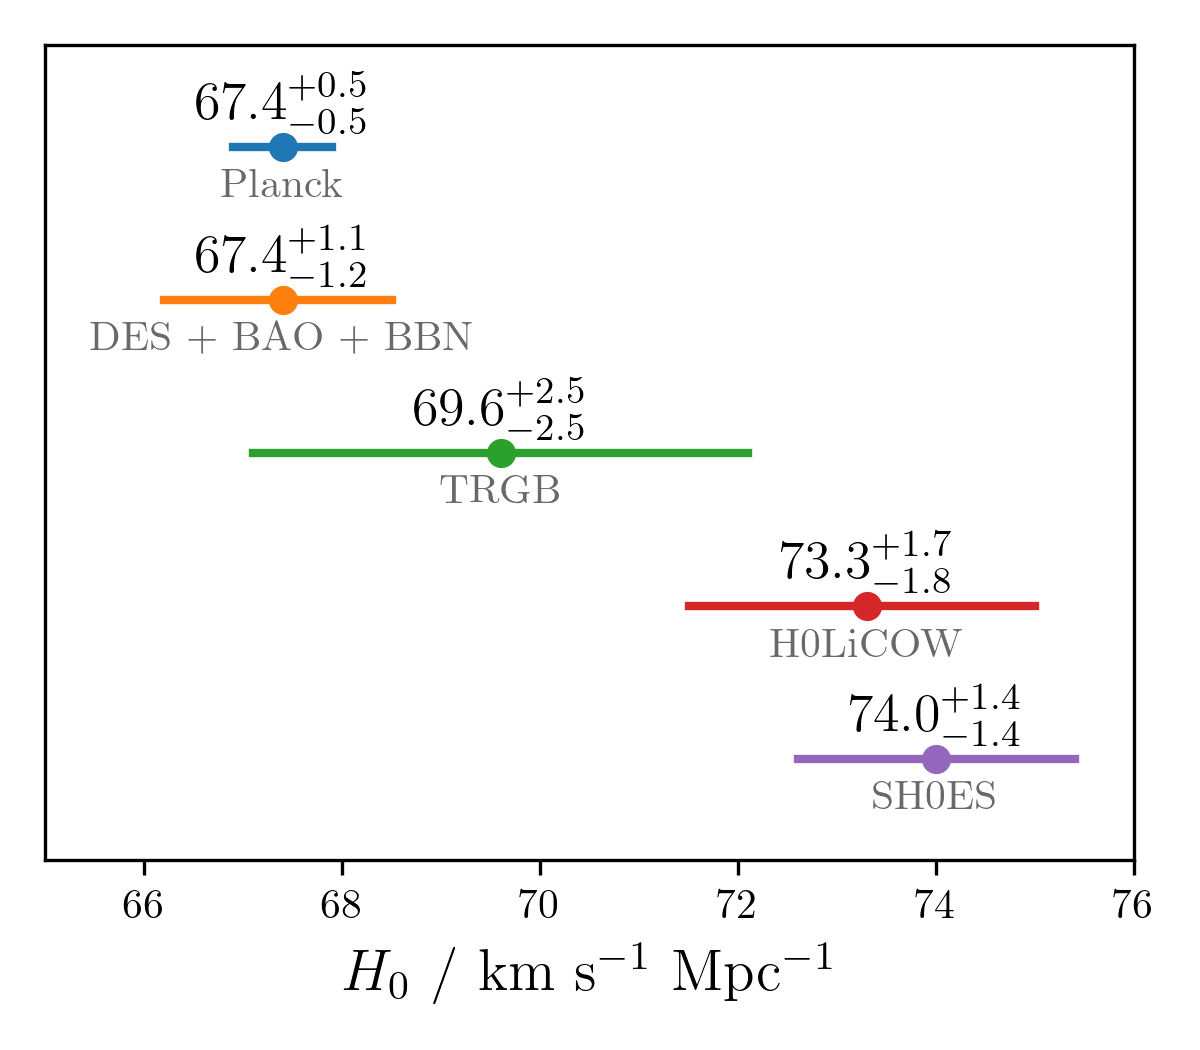
\includegraphics[width=0.8\columnwidth]{../plots/H0 tension.png}
    \centering
    \label{H0_tension}
    \caption{A compilation of recent measurements of the Hubble constant $H_0$. The top two measurements are from early-universe datasets using $\Lambda$CDM cosmology \cite{Planck2020, Abbott2018}, while the remaining three are from late-universe datasets based off local distance ladder measurements \cite{Freedman2020, Riess2019, Wong2019}. The tension between the Planck and SH0ES measurements currently stands at $4.7 \sigma$.}
\end{figure}


In addition to the Hubble constant, less severe tensions also exist. Discrepancies of $3\sigma$ have been reported with respect to the matter density $\Omega_m$ and rate of growth of structure $\sigma_8$, between the Cosmic Microwave Background (CMB) data collected by Planck and the weak lensing-based Kilo Degree Survey (KiDS) \cite{Heymans2021}. There has also been arguments made for the existence of a "curvature tension", with inconsistencies of $2.5 \sigma$ to $3 \sigma$ between CMB data alluding to a closed curved universe and the tenet of flat curvature in $\Lambda$CDM cosmology \cite{Handley2021Closed}.

These tensions raise questions surrounding the validity of the well-established, well-tested standard cosmological model -- the $\Lambda$CDM. Are these tensions just an artefact of systematic errors from collecting and analysing datasets? Or do these tensions hint at something more fundamental -- perhaps a modification to the standard model, or more excitingly new physics to take the place of the old one?

However, before we make that leap into the realm of new physics, it is essential for us to examine how tension is quantified. With cosmological datasets being multi-dimensional, the problem of quantifying discrepancies is non-trivial. Datasets that appear to be in mild tension, such as the DES Y1 and Planck datasets, have been reported to be consistent when using the canonical Bayes factor $R$ \cite{Handley2019}. This is troubling, and is a reflection of the difficulty of the problem. With tensions likely to increase as measurement precision increases, a variety of tension metrics have been proposed in recent literature \cite{Charnock2017} to better understand the problem at hand.

This paper aims to develop on the idea of maximum tension. With cosmological datasets, larger tensions often exist across multiple parameters rather than within each parameter on its own. A good example would be the $3 \sigma$ tension between $\Omega_m$ and $\sigma_8$ -- the tension is obvious in a two-dimensional plot between these two parameters, but is non-existent when the parameters are inspected individually. In a high-dimensional parameter space, it is thus likely that there exists a combination of parameters which exacerbates and maximises tension.

In this paper, we explore how a high-dimensional parameter space can be mapped onto a \textit{tension coordinate} -- a lower-dimensional coordinate which maximises the tension between two datasets. A neural network is used to achieve this mapping, since the non-Gaussian nature of certain cosmological parameters renders an analytical approach challenging. This tension coordinate is then applied to the Planck and DES Y1 datasets. Such an approach could allow us to develop a better intuition of the source of tension, and verify the large tensions that currently exist in $H_0$ and the $\Omega_m$-- $\sigma_8$ plane.


\section{Background}

Despite certain pitfalls \cite{Handley2019} of the Bayes Factor R \cite{Marshall2006}, 



\section{Method}

\section{Results and Discussion}

\section{Conclusions}





\begin{acknowledgments}

\end{acknowledgments}

\appendix

\section{Appendixes}

\section{A little more on appendixes}


\subsection{\label{app:subsec}A subsection in an appendix}




% The \nocite command causes all entries in a bibliography to be printed out
% whether or not they are actually referenced in the text. This is appropriate
% for the sample file to show the different styles of references, but authors
% most likely will not want to use it.

\bibliography{apssamp}% Produces the bibliography via BibTeX.

\end{document}
%
% ****** End of file apssamp.tex ******